\documentclass[../main.tex]{subfiles}
\begin{document}
\section{Introduction}
In the last 50 years car have transitioned from being composed only by mechanical parts to being completely stacked with electronics. The complexity of vehicles arises every year and the industry continuously raise the bar on the state of the arts. The transitions to electro-mobility, the ADAS systems have done all but slowing down the development. The more a topic is market relevant, the higher the competition between companies, the faster the development in that field is going to be. The automakers are always ready to exploit or create new needs in order to adapt and attract customers. Automotive pulse of innovation and the "German Silicon Valley" is the place a engineer want to be to fell part of this complex, but for sure perfectly oiled, machine.   
\begin{figure}
\centering
\begin{minipage}{.5\textwidth}
  \centering
  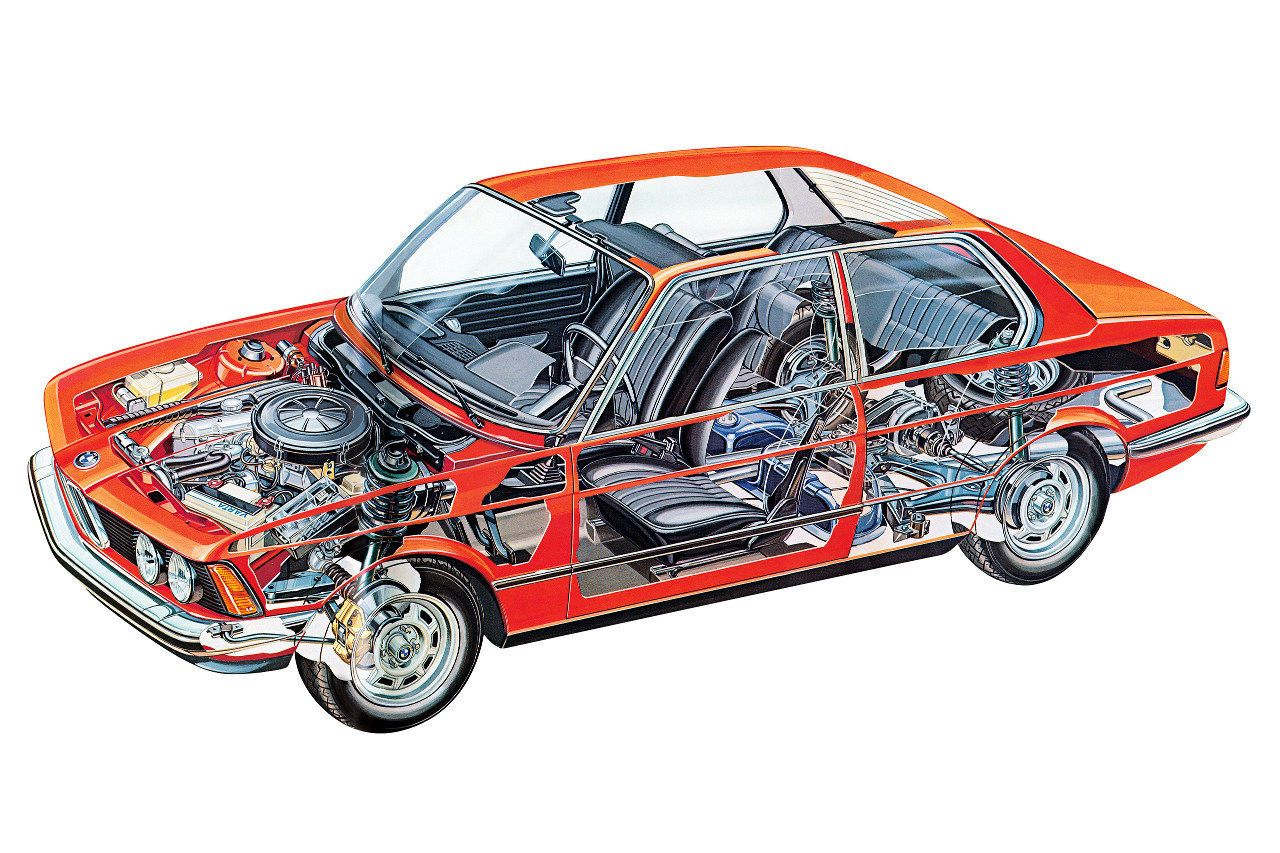
\includegraphics[width=\linewidth]{images_folder/4a56e1d50b56da42a10e29d451cf2b93.jpg}
  \caption{BMW 320 Coupe E21 - 1975}
  \label{fig:test1}
\end{minipage}%
\begin{minipage}{.5\textwidth}
  \centering
  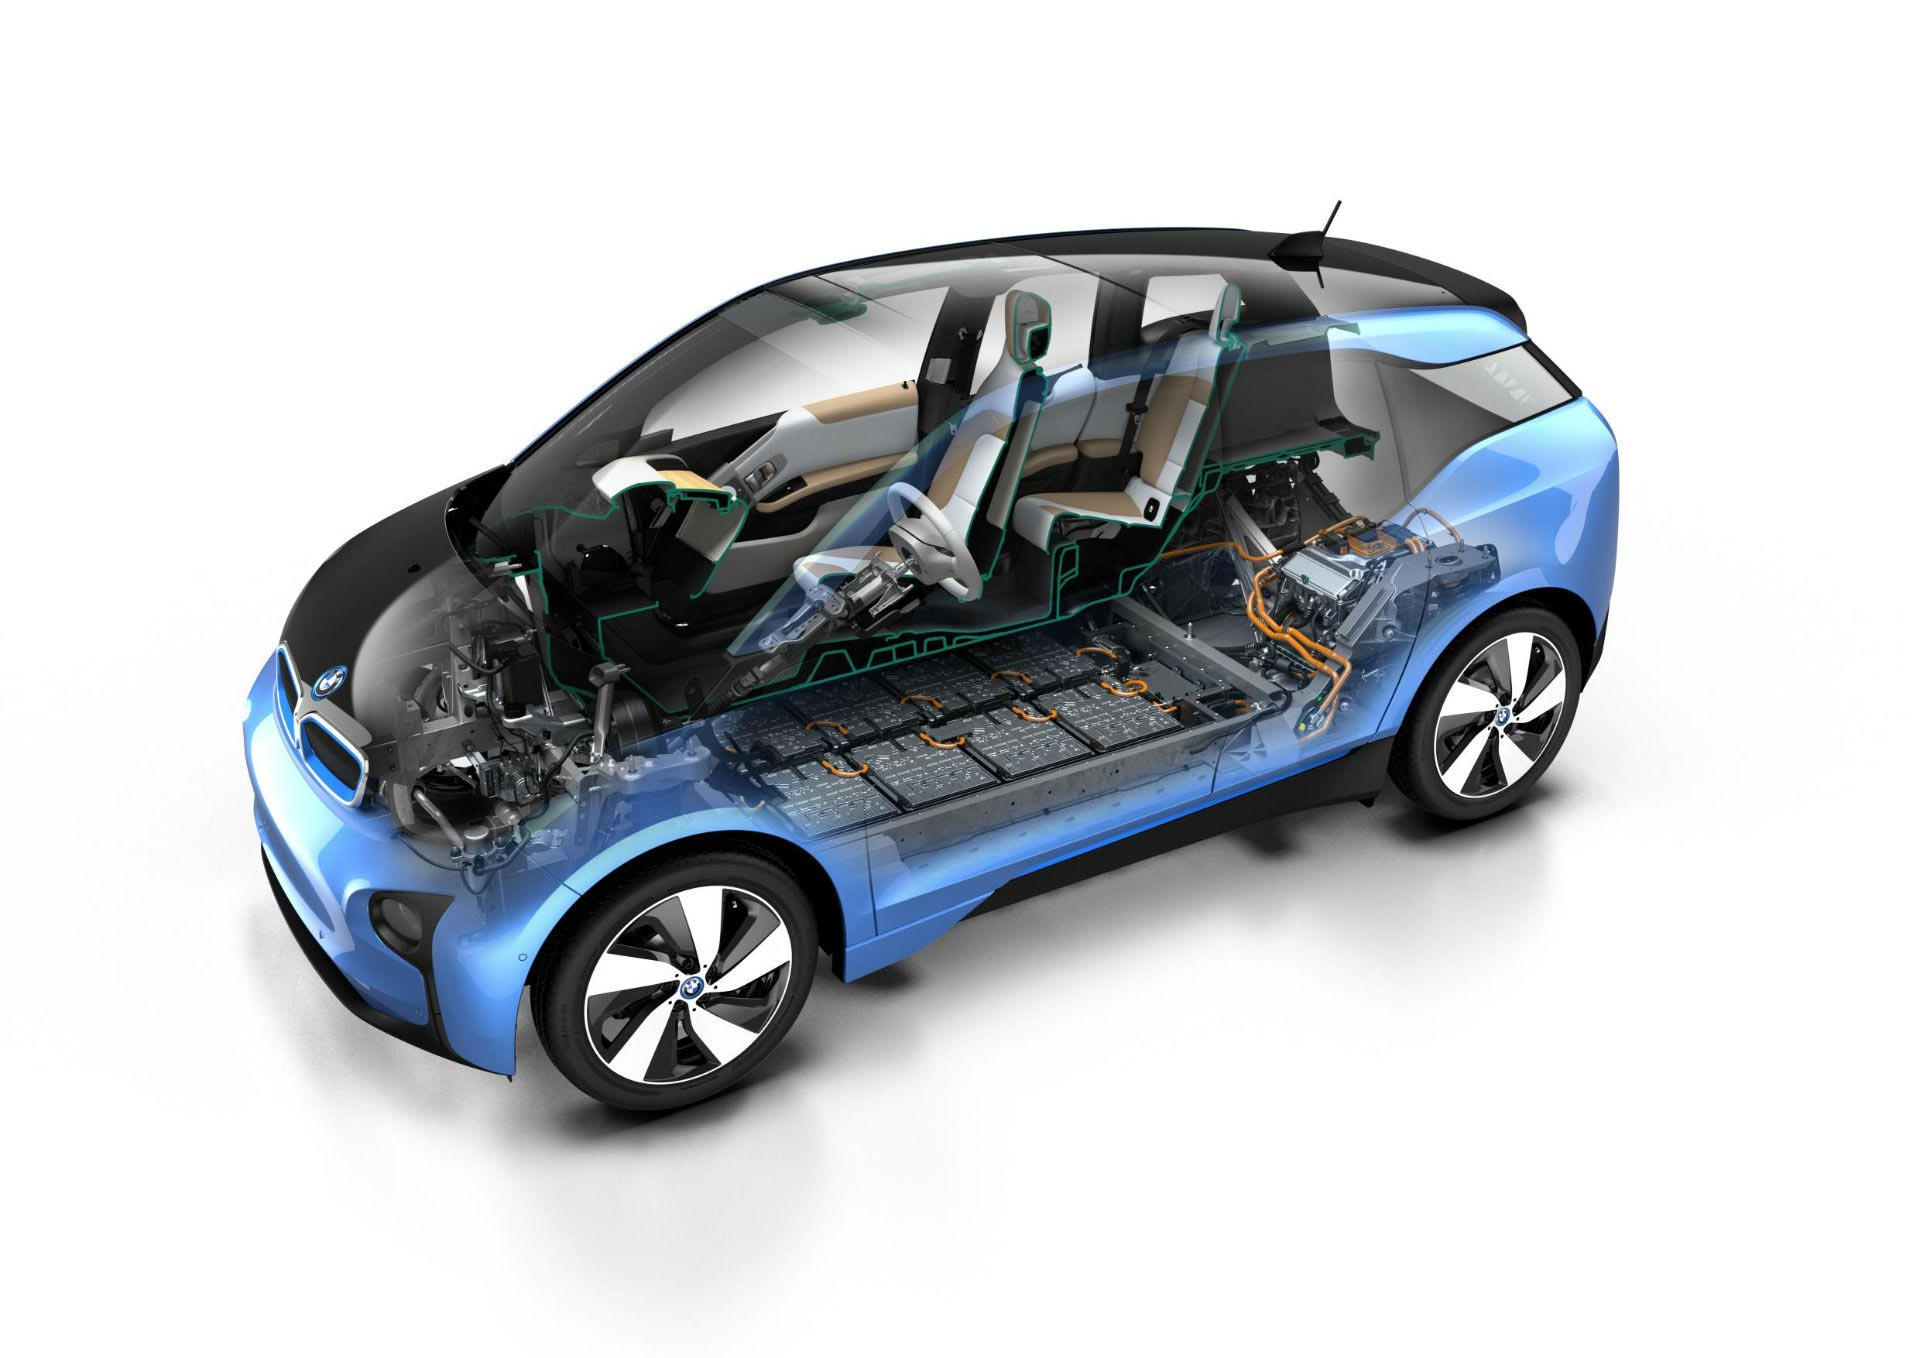
\includegraphics[width=\linewidth]{images_folder/BMW_i3.jpg}
  \caption{BMW I3 - 2015}
  \label{fig:test2}
\end{minipage}
\end{figure}

\section{Block Schema of a car}
The complexity of system car can be easily simplified by block schemes. Block schemes are going to be a recursive topic during the thesis, thanks to the outside view that allow to have on complex topics. 

The input to the system car can be an array of driver commands, such as the steering position, accelerator pressure and all the switches that control the car. The output of the system is the movement of the car, the feedback loop report to the user not only the position in space but also other feedback parameter as the drive comfort or more simply if the light of the headlight is enough for the lighting the road. The complex black box car can then inspect further. Inside the system car we can identify two main blocks. The mechanical one and the electrical one. We can see how feedback loop start to intersect with each other. The electronics drive the mechanics which output is taken back from the electronic to better the response. The system car can be considered a complex version of an embedded system where electronics drive mechanics following a logic stored in a CPU under the guise of code lines. 


\cleardoublepage
\end{document}